% 
% Annual Cognitive Science Conference
% Sample LaTeX Paper -- Proceedings Format
% 

%% Change "letterpaper" in the following line to "a4paper" if you must.

\documentclass[10pt,letterpaper]{article}

\usepackage{cogsci}
% Recommended, but optional, packages for figures and better typesetting:
\usepackage[margin=1in]{geometry} 
\usepackage{microtype}
\usepackage{graphicx}
\usepackage{subfigure}
\usepackage{booktabs} % for professional tables
\usepackage{nicefrac}       % compact symbols for 1/2f, etc.
\usepackage{microtype}      % microtypography
\usepackage{float}
\usepackage[colorlinks,allcolors=purple]{hyperref}
\usepackage{algorithm}
\usepackage{amsmath}
\usepackage{graphicx}
\usepackage[table,xcdraw]{xcolor}
\usepackage{gensymb}
\usepackage{stmaryrd}
\usepackage{amssymb}

%\cogscifinalcopy % Uncomment this line for the final submission 


\usepackage{pslatex}
\usepackage{apacite}


%\usepackage[none]{hyphenat} % Sometimes it can be useful to turn off
%hyphenation for purposes such as spell checking of the resulting
%PDF.  Uncomment this block to turn off hyphenation.


%\setlength\titlebox{4.5cm}
% You can expand the titlebox if you need extra space
% to show all the authors. Please do not make the titlebox
% smaller than 4.5cm (the original size).
%%If you do, we reserve the right to require you to change it back in
%%the camera-ready version, which could interfere with the timely
%%appearance of your paper in the Proceedings.



\title{Contextually-adapted abstractions explain \\ contextually-adapted abstraction in language} 
 
\author{{\large \bf Morton Ann Gernsbacher (MAG@Macc.Wisc.Edu)} \\
  Department of Psychology, 1202 W. Johnson Street \\
  Madison, WI 53706 USA
  \AND {\large \bf Sharon J.~Derry (SDJ@Macc.Wisc.Edu)} \\
  Department of Educational Psychology, 1025 W. Johnson Street \\
  Madison, WI 53706 USA}


\begin{document}

\maketitle


\begin{abstract}
A crucial dimension in communication is the level of abstraction at which people pitch their language.
While we do flexibly shift our words to suit the needs of different contexts, the ways in which we do so when describing compositional phenomena is less well understood.
In this paper we present a novel set of hierarchical stimuli, and present an experiment in which we elicited compositional descriptions of these stimuli in different contexts. 
We compare participants' descriptions to \textit{a priori} and learned measures of the formal structure of these stimuli, allowing us to assess the extent to which context shifts the level of abstraction reflected in participants' words.

\textbf{Keywords:} TBD
\end{abstract}


\section{Introduction} \label{sec-introduction}
\begin{enumerate}
    \item Main question: Language isn’t a monolith -- people can choose many different ways to describe the exact  same thing. What explains that variation in language? Specifically, we focus on grounded language that is about things in the world -- \textbf{what explains the set of concepts people choose to convey that thing, and in particular, what determines the level of abstraction that they choose?}
    \item Prior work (eg. Tian) has demonstrated that people perceive and quickly learn abstract domain structure - in particular, that they are attentive to the set of abstract concepts used to carve up the space, and that the way they parse images drawn from a generative model is consistent with the optimal concept library fit to the stimuli they observe.
    \item We hypothesize that this is reflected in language -- that people produce language that reflects an abstract, domain-specific concept library. 
    \item We adopt the more formal modeling hypothesis in (LOT, Tian, McCarthy, Wong, others): that people represent underlying domain-structure in a compositional, language-like LOT, and specifically, a domain-specific concept library with program-like structure. Therefore, our hypothesis can be evaluated by looking for correlations in the language produced and underlying programs, drawn from differing formal DSLs at different levels of abstraction.
    \item To evaluate this:
        \begin{enumerate}
            \item We collect a corpus of grounded language in which this can be studied systematically in two domains (Section \ref{sec-dataset}), comprised of two domains with hierarchical structure in how the stimuli vary, and permitting multiple levels of abstraction - in which we have access to differing ground truth DSLs that generate the stimuli.
            \item We first compare a base DSL of low-level parts to two increasingly higher order DSLs and find that the language people produce is better explained by a higher-order, part-based concept library (Section B.)

        \end{enumerate}
\end{enumerate}


\begin{figure*}
  \begin{center}
  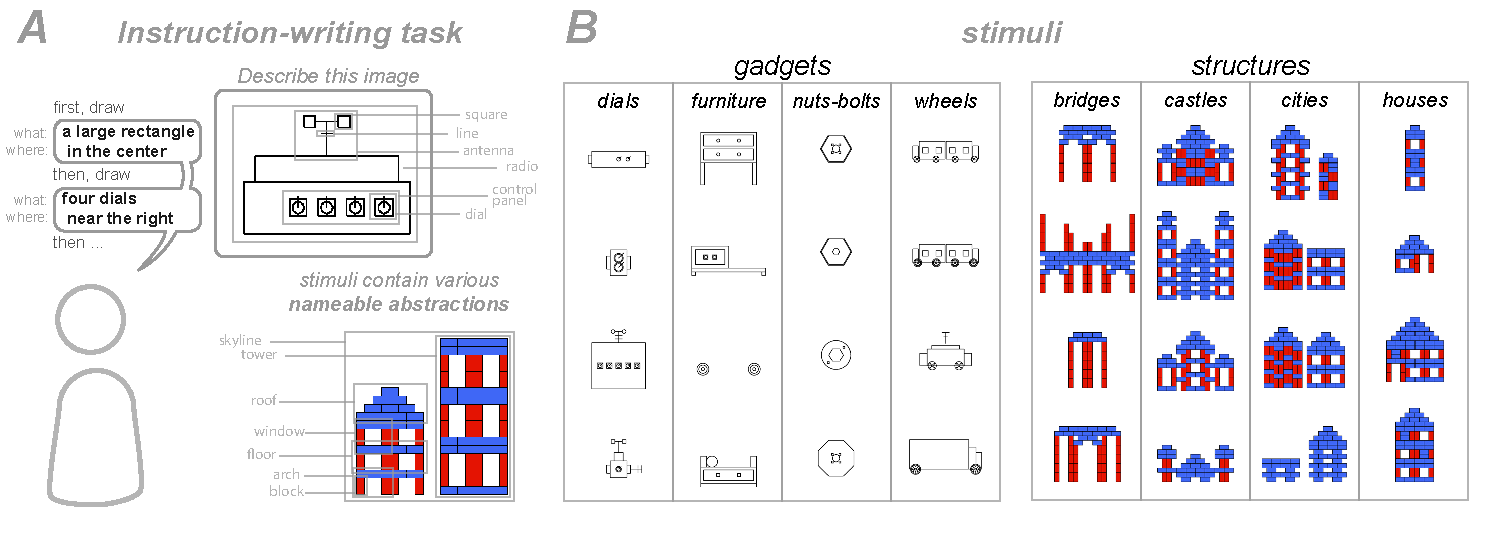
\includegraphics[width=0.99\linewidth]{figures/task_fig_full.pdf}
  \caption{}
  \label{fig:task}
  \end{center}
  \end{figure*}    

\section{Part I: Domain context influences vocabulary choice} \label{sec-part-i}
% Can we have a running example here?
Consider how you might describe the drawing or block tower in Figure \ref{fig:task}A. Both images could be described in language that carves up the image, intuitively, at multiple levels of abstraction -- how would you choose between describing the drawing using a simple but low-level vocabulary of basic strokes (like \textit{lines, circles, and squares}) vs. a set of names for some of its functional parts (like \textit{antenna} or \textit{dial}); or between describing the block tower as composed of \textit{red blocks} and \textit{blue blocks} vs. of higher-level parts like a \textit{roof} and \textit{floors}?

Our first goal was to investigate the basic claim that people can adapt the linguistic vocabularies they use to describe visual objects like these contextually, based on the distribution of objects they intend to describe. To accomplish this, we construct two domains of stimuli (\textit{gadgets} and \textit{structures}) (Fig. \ref{fig:task}B) that are generated from a shared base set of procedural, symbolic primitives, but that vary hierarchically subdomains in terms of their compositional parts. We then run a language production experiment to elicit language from subjects familiarized with stimuli from a specific subdomain. We hypothesized that the vocabularies people used to describe each stimulus would be \textit{context-specific}: that participants would tend to use different vocabularies tailored to the sub-domain distribution of stimuli they were shown.


\subsection{Methods: Language production experiment}



% \begin{enumerate}
%     \item Describe stimuli generation : two domains (gadgets; towers); four subdomains in each.
%     \item Describe language generation task.
% \end{enumerate}
\paragraph{Hierarchical stimulus generation} % two domains (gadgets; towers); four subdomains in each.

% todo: tie to program abstraction
% Desiderata: 1) varied set of categories, 2) hierarchical structure; 3) primitives + higher-order abstractions available to describe, 4) novel + evocative

% 	What do these buy us?
% #1 more general findings
% #2 reminiscent of hierarchical structure of real-world concepts
% #3 allows us to test the notion of "basic-level" but for parts (Rosch et al.) (“just right” level of abstraction)
% #4 lets us look at learning (later)

% 'structures' :  ['bridge', 'castle', 'house', 'city'],
% 'drawing' :  ['nuts-bolts','wheels','furniture','dials']

To investigate how the compositional structure of an object's domain affects the language people use to describe that object, we designed a collection of artificial image stimuli that were hierarchically constructed from smaller parts  (Fig. \ref{fig:task}B).
% Different primitives (i.e. difference between domains)
Our stimulus set consisted of two distinct domains that were each procedurally generated from a set of base primitives.
\textit{Gadgets} were designed to resemble technical drawings of functional objects, and were composed of digital pen strokes.
\textit{Structures} were designed to resemble architectural structures, and were composed of horizontal and vertical blocks.
Each item corresponded to a generative program involving the base primitives of its domain. 
Critically, each domain involved a set of mid-level abstractions  (e.g. \textit{wheels}, \textit{roofs}) that could appear across different stimuli. 

% Different compositional structure within domain (difference between subdomains)
Furthermore, each domain was further subdivided into four subdomains, which were each defined by a distinct generative procedure that was hand-designed to produce objects of a recognizable subordinate category (e.g. \textit{furniture}, \textit{castle}) from a set of predefined abstractions (e.g. \textit{legs}, \textit{tower}).
Several of these abstractions were shared between subdomains (\textit{roofs}, for example appeared in both \textit{houses} and \textit{skyscrapers}), which allowed us to compare the language used to pick out abstraction types in different contexts.
We enumerated all possible stimuli for each subdomain, and selected a random but biased sample of each to obtain 250 stimuli of varying size for each subdomain.


\paragraph{Procedural language production task}

% procedural
To evoke a thorough decomposition of each object's component parts, we asked participants to produce a complete sequence of instructions for constructing each stimulus.
Each participant produced instructions for 10 items from a single \textit{subdomain} (e.g. only \textit{castles}), either describing how to ``draw'' the item if describing a subdomain of \textit{gadgets}, or how to ``build'' the item if it was a \textit{structure}.
% what/where framing
To disentangle referring expressions from spatial information, we provided an interface in which participants could enter step-by-step instructions, where each step involved typing \textit{what} would be placed/drawn \textit{where} in separate ``what'' and ``where'' text boxes (Fig. \ref{fig:task}A).
Participants could add as many instruction steps as they liked, and had no time limit.

% familiarization and design
To familiarize participants with the kinds of stimuli and abstraction that could appear in their subdomain, they were first required to click through images of 25 other stimuli from their subdomain, disjoint with the set to be described. 
While describing each image, they could also see up to 7 of the upcoming stimuli.
We collected data from participants until all (2 domains * 4 subdomains * 250) stimuli had been described by at least 2 participants with complete datasets (i.e. had described all 10 of their items).
% \todo{how many participants did we collect in the end? how many descriptions?}
Participants were paid around \$15 per hour for their time. 

\begin{figure*}
  \begin{center}
  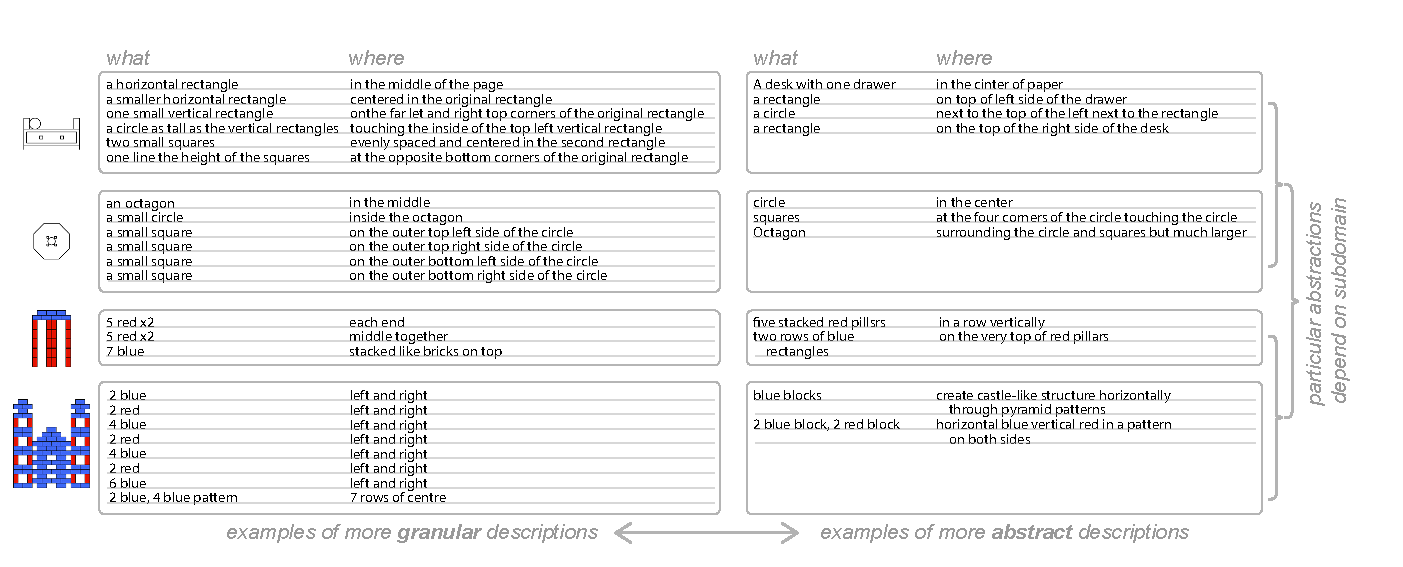
\includegraphics[width=0.99\linewidth]{figures/instruction_examples.pdf}
  \caption{Examples instructions written by participants. Some, more granular descriptions (left) referred to the base primitives (strokes and blocks); others referred to higher-level constructs that combined multiple of these primitives. Differences between language can be seen between domains, but also within a single domain at the subdomain level.}
  \label{fig:intruction_examples}
  \end{center}
  \end{figure*}

\paragraph{Language preprocessing} % spacy, en_core_web_lg,
To better investigate the content of the instructions generated by participants, we use the spaCy NLP library to extract and lemmatize words. %, as well as remove stop words.

% Add TF-IDF filtering?

% \subsection{People use different words for different domains and subdomains} 

% people use abstractions at all


\subsection{Results}
% ($b=XXX$, $t=XXX$, $p=XXX$)
% $XXX\%$ (95\% CI: $[XXX, XXX]$)

% descriptive statistics of dataset
We collected 4961 sets of instructions from a total of 589 participants. %TK: recalculate
%465 participants completed their set of 10 annotations.
Instructions produced for \textit{castles} tended to be longer than those for \textit{gadgets}, both in terms of the number of instruction steps provided ($b=XXX$, $t=XXX$, $p=XXX$) and the raw character counts ($b=XXX$, $t=XXX$, $p=XXX$).
Nevertheless, it appeared that instructions produced for both domains spanned a range of levels of abstraction (Fig. \ref{fig:intruction_examples} left vs. right), where some referred to lower level primitives (i.e. geometric shapes and individual blocks) and some to more abstract compositions of these lower elements (e.g. ``desks'', ``pillars'', and ``castle-like structures'').
Stimuli from each domain, however, were constructed from distinct sets of base primitives that can be combined according to distinct sets of constraints, allowing us to investigate whether participants systematically varied their vocabulary according to their context.

\paragraph{Domain-specific abstraction in language}
To explore any systematic differences in the vocabularies used for each domain, we calculated the TF-IDF score of each word for each domain, visualizing the most diagnostic words from domain (Fig. \ref{fig:intruction_examples} A). % can't be used to say that there is a difference between domains
This revealed a range of both lower-level (``red'',``blue'',``circle'',``diameter'') and higher-level (``wheel'',``drawer'',``stack'',``pyramid'') concepts that were diagnostic of each domain.

\begin{figure}
  \begin{center}
  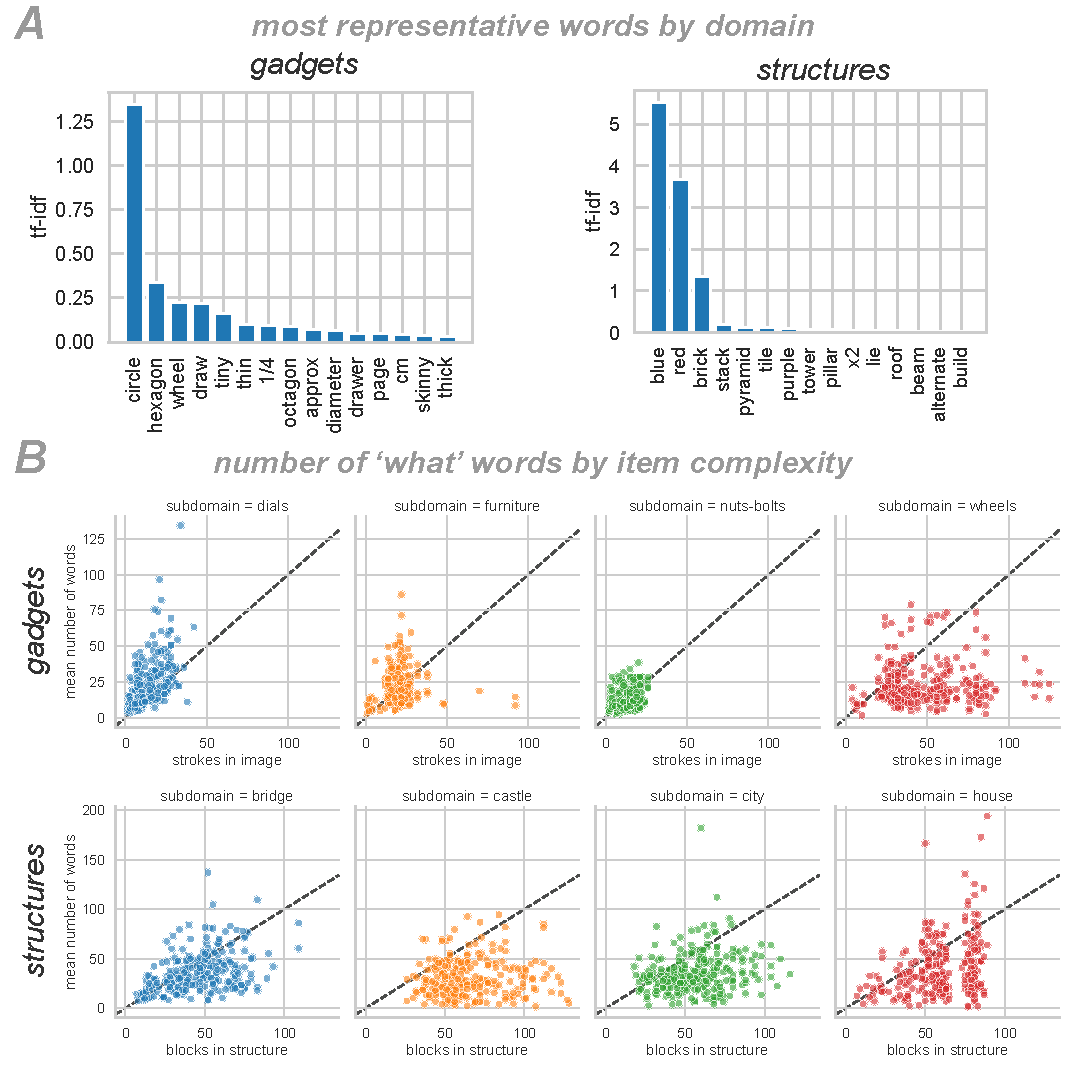
\includegraphics[width=0.98\linewidth]{figures/words_domain_subdomain.pdf}
  \caption{A) Domain-specific words used to write instructions. B) Number of words in \textit{what} text-boxes was correlated with complexity of structures, but sub-linearly, suggesting that higher-level abstractions were used to refer to collections of primitives.}
  \label{fig:words_results}
  \end{center}
  \end{figure}

\paragraph{Subdomain-specific abstraction in language}
We also designed our stimuli to include several subdomains containing different abstractions over the base primitives used to construct items in the domain.
Did the instructions produced by participants reflect these differences in subdomain structure?
[todo:per-subdomain td-idf histogram. Do some subdomains have fewer distinctive (high tf-idf) words i.e. do people rely on lower-level primitives in some subdomains? (motivate upcoming sections).]


\section{Part II: Language complexity correlates non-linearly with base primitive complexity} \label{sec-part-ii}
Each stimulus in Sec. \ref{sec-part-i} can be represented with its generating program in a base DSL of low-level primitives (\textit{strokes} in gadgets; \textit{blocks} in structures) shared across the domain. Before considering more abstract representations, we can first ask: do these underlying program representations at all predict the language people use to describe each stimulus? We conduct a control experiment to establish an initial correspondence between the procedural program representations in the base DSL and human language, by correlating \textit{program description length} (program token counts) in the base DSL with \textit{language description length} (language token counts.)  

We hypothesized a positive, but non-linear, correlation between description lengths in the base DSL and human language: we expect that even when measured in low-level primitives, more complex stimuli should require more words to describe; but we also expect that the existence of domain-specific abstractions named in language (as established in Section I) should mean that people's language length should not scale linearly with the number of blocks or strokes in each stimulus.
We found that instruction length did correlate with complexity (Fig. \ref{fig:words_results} B), and that this correlation was, in general, sub-linear. % does this mean something different from gradient < 1?
Furthermore, we found that the extent that this was true varied by subdomain, with some subdomains yielding stronger correlations between the instruction length and number of base primitives. %change this to linear model?
This suggests that participants are utilizing the abstraction structure of the domain they are describing.

\section{Part III: Contextually-adapted abstractions can better predict language production}\label{sec-part-iii}
Our results so far suggest that people adapt the vocabularies they use to the context of the subdomain they described (Part I); and that there is a positive, but non-linear, correspondence between the linguistic descriptions of each stimulus and their \textit{generating program} in the base DSL shared across each domain. In this section, we now ask whether we can better explain the language people used in each subdomain using \textit{contextually-adapted} DSLs containing higher-level abstractions than these base primitives. 

We introduce a method for contextually varying the level of DSL abstraction used to represent the generating program for each stimulus, by enriching the initial base DSL of primitives with program abstractions that capture context-specific parametric variation within each subdomain. We also introduce a richer, model-based correlation metric between programs and language for each stimulus, based on a statistical program-to-language model fit to the language data in each domain. Using this, we first hypothesize that generative programs rewritten using \textit{contextually-specific abstractions} should better predict language than the initial base primitives.

However, we also hypothesize that speakers take into account the underlying \textit{vocabulary size} as a representational cost for describing the domain as a whole -- a speaker incurs the cost of using an increasingly large, and increasingly arcane, vocabulary of unique concepts as they consider additional context-specific abstractions to describe any one stimulus. Our model formalizes this cost explicitly: increasing the level of DSL abstraction increases the DSL size, as more and increasingly complex program abstractions are added to the small set of initial base primitives. Concretely, we expect the correlation between programs in the base DSL and language to increase only to an intermediate level of abstraction, and then decrease, yielding a characteristic U-shaped curve indicating this tradeoff.


% However, our model also suggests an intriguing additional representational cost for speakers across the subdomain as a whole. Consider the difference in re-describing the technical drawing in (Fig. 1A) using increasingly contextually-abstract vocabularies: from the base primitives (as a set of \textit{squares, circles, and lines}), to an intermediate set of contextual abstractions (such as \textit{antennas} or a \textit{dials}), to an extremely high-level and contextually-specific vocabulary (such as one that includes a name like \textit{model-7000} that exactly identifies that particular image.) While the description for any particular stimulus grows more concise, intuitively, this comes with a tradeoff in the overall unique vocabulary size across the subdomain: a speaker must introduce more, and more arcane, words for each high-level concept. Our model formalizes this explicitly: increasing the level of DSL abstraction increases the DSL size, by adding more and increasingly complex abstractions to the small set of initial base primitives.

% We hypothesize that this cost will be reflected in how well DSLs at increasing levels of abstraction predict speaker behavior: we expect to see a characteristic, inversely U-shaped curve when correlating DSLs at increasing levels of abstraction (and of increasing sizes) with language. % This is stated clunkily.

% Our results so far suggest that people use cually-adapted vocabularies to describe stimuli (Part I); and that the lowest-level, base primitive representation of each object only partially explains the words a person needs to describe it -- in particular, people are often able to describe an object using fewer words than the base primitive representation would predict (Part II). Taken together, an intuitive explanation for these results is that -- while a person could in principle use the exact same vocabulary of low-level base concepts to describe any given stimulus in the domain -- they instead a vocabulary of higher-level, context-specific abstractions adapted to the specific subdomain they were asked to describe.

% Our formal modeling hypothesis in (Part II) correlated language with stimulus representations written in a base DSL of simple primitives shared across each domain. In this section, we present a method for \textit{contextually-adapting} the DSL to the subdomain; and for \textit{varying the level of contextual abstraction} in the DSL based on parametric variation in the underlying generative process for each subdomain. We also introduce a richer correlation metric between program representations and linguistic descriptions for each stimulus based on a statistical program-to-language translation model. Concretely, we evaluate how well program representations in varying DSLs explain language based on $P(language | program, \mathcal{L})$ in a statistical program-language translation model, where $\mathcal{L}$ is a particular DSL and $P(language | program, \mathcal{L})$ is the predictive likelihood of a linguistic stimulus description given its program. We first hypothesize that contextually-adapted DSLs should better explain contextual language: we expect higher $P(language | program, \mathcal{L})$ for a contextual DSL adapted to each subdomain than the raw base primitives.


\subsection{Methods: Identifying language abstraction with varying levels of program abstraction}
\paragraph{Generating DSLs at varying levels of abstraction} As described in Part I, stimuli in each subdomain are generated procedurally using nested levels of recursive, parametric variation: for instance, the \textit{dials} stimuli are generated first by nesting sets of primitive shapes in the base DSL to create \textit{dial} parts, which are themselves repeated and translated to create the \textit{rows of dials} in many of the images. Similarly, the \textit{house} stimuli are generated by first composing the blue and red block primitive shapes to create higher-order \textit{window} and \textit{brick} parts, which are tiled to create individual \textit{floors}, which are themselves stacked to create entire \textit{walls}. 

% This parametric variation is context-specific, with increasing context-specificity at increasing levels of abstraction (Fig. \ref{fig:lanuage_libraries} A): for instance, in contrast to the \textit{dials} domain, for instance, base primitives in the \textit{furniture} domain are first used to generate individual \textit{handles, drawers, and legs}; then into \textit{rows of handles, stacks of drawers, and sets of legs}; and finally into entire  \textit{bookshelves} or \textit{lounges}.

Using the underlying procedural generative model for each subdomain, we therefore introduce contextual program abstractions into the base DSL -- and re-represent the generative program for each stimulus using these abstractions -- at three increasing levels of abstraction, corresponding to nested parametric variation over parts. These levels of abstraction, while driven by the underlying generative procedure, are chosen manually based on parametric depth -- clearly, there are more than three possible levels of variation in each domain. Future work can investigate additional possible levels of abstraction, as well as bottom-up methods for automatically discovering these abstractions and re-writing the generative programs from their base primitives (as in [CITE Ellis]).

We choose to separately consider DSLs at each level abstraction both with and without the numeric parameters that parameterize each stimulus. In total, we consider the following DSL representations, ordered by their DSL size (the number of unique program tokens across the full subdomain):
\begin{itemize}
    \setlength\itemsep{0.1em}
    \item \textbf{Base DSL}: the low-level shared primitives (strokes and blocks) across the full domain.
    \item \textbf{$L_1$}: a  DSL corresponding to first-order parametric variation (eg. lines rotated into polygons)
    \item \textbf{$L_1$ with parameters}: the DSL with added tokens for numeric parameters (eg. the scaling constants for individual polygons.)
    
    \item \textbf{$L_2$}: a  DSL corresponding to intermediate parametric variation (eg. polygons nested into 'dials')
    \item \textbf{$L_2$ with parameters}: the DSL with tokens for numeric parameters (eg. the number of nested polygons.)
    
    \item \textbf{$L_3$}: a DSL corresponding to high-level parametric variation (eg. specific 'bases' with varying dials)
    \item \textbf{$L_3$ with parameters}: the DSL with tokens for numeric parameters (eg. the number of dials.)
\end{itemize}

Fig. \ref{fig:language_libraries}A shows sample visualized components from these three increasingly abstract DSLs ($L_1$, $L_2$, $L_3$) along with the initial shared base DSL. We also release the full generative procedure (including the abstraction re-generation) in the code repository.

\paragraph{Correlating program abstractions with language} In Part II, we measured correspondences between program representations of stimuli and language descriptions using a simple description length metric. Here, however, we are interested in correlating specific programmatic concepts  -- components in a given DSL that are composed to generate each image -- with particular linguistic concepts -- words and phrases composed to describe each image. Therefore, we introduce a richer model-based metric based on \textit{statistical translation models} fit to predict linguistic descriptions from generating programs.

Specifically, given a particular DSL $L$, we consider the \textit{heldout predictive likelihood} $P(description | program, L)$ over heldout batches (n=5) of stimuli  by fitting the program-to-language translation model to all but the heldout set of stimuli, and then evaluating the model on the heldout stimuli. We use the statistical translation model known as IBM Model 1 \cite{gal2013systematic}, which directly estimates token-token alignments between programs and language.

Figure \ref{fig:language_libraries}B. shows log perplexity in the translation model (mean log likelihood of predicting language tokens from program tokens, which normalizes for length of the linguistic description) for models fit to programs in varying DSLs, ordered by their DSL size (which corresponds to increasing levels of abstraction -- as discussed earlier, higher levels of contextual abstraction introduce more context-specific program components.)

\begin{figure*}[h]
  \begin{center}
  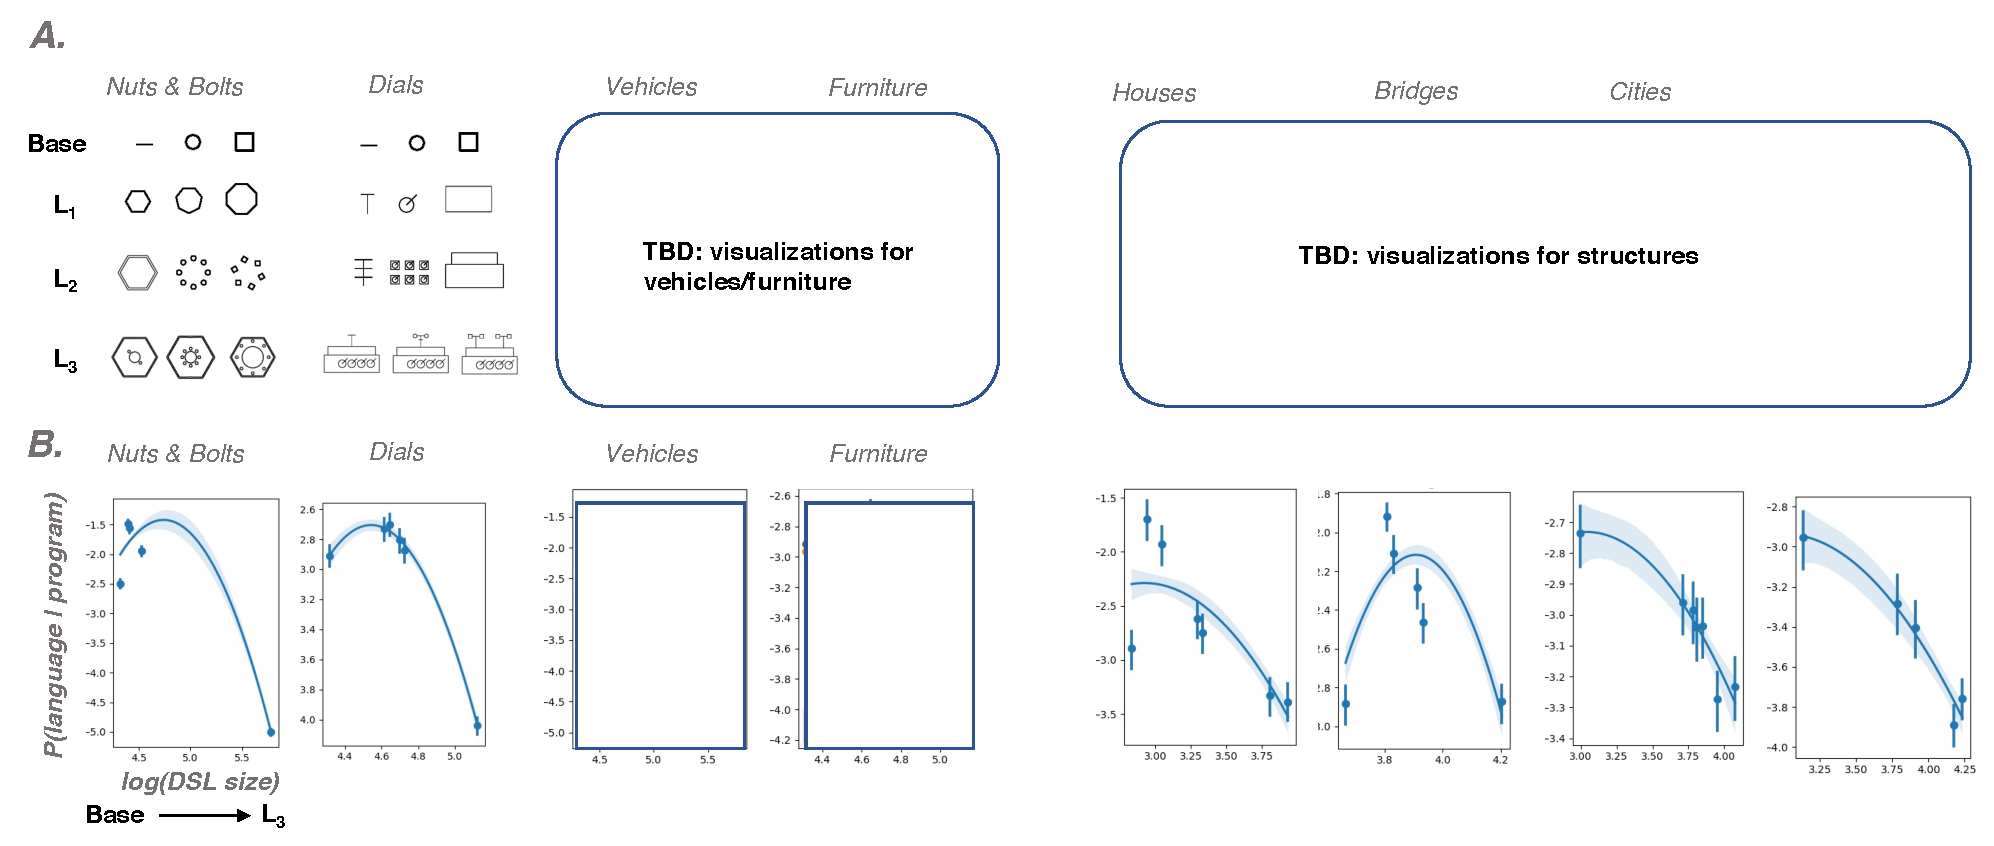
\includegraphics[width=0.99\linewidth]{figures/fig_language_libraries.pdf}
  \captionenerating 
  \label{fig:language_libraries}
  \end{center}
  \end{figure*}
 
\subsection{Results}

\paragraph{People adapt the abstractions they use contextually to the subdomain.} We hypothesized that higher-level DSLs, containing context-specific abstractions, would always better predict language in each subdomain. Our results in Fig.  \ref{fig:language_libraries}A suggest that this is generally true, along with a more nuanced interpretation: in \textit{most} of the subdomains, a contextual DSL improves perplexity under the translation model as compared to the base DSL. However, in two of the structures subdomains --  the \textit{cities} and \textit{castles} domain, in fact the base DSL yields the best perplexity. 

This result suggests that people do indeed adapt the level of abstraction they use in language, dependent contextually on the subdomain of stimuli -- after all, while the base DSL can be used to describe \textit{every} subdomain (eg. people could \textit{always} have described each structure in terms of its low-level blocks), people seem to have chosen it selectively for some domains and other, more context-specific abstractions for others.

What explains when people fall back on the base DSL of primitives? A visual inspection of the \textit{cities} and \textit{castles} abstractions suggests one intuitive explanation: the availability of commonly-understood linguistic terms to describe these abstractions. While our results in many domains suggest that people flexibly pick out higher-level, contextual abstractions -- and adapt their vocabulary to reflect them -- humans performing a naive procedural description task, intended for other naive speakers, are also constrained by the basic English terms available to them. We see these results as especially promising for ad-hoc \textit{convention formation} paradigms [CITE], to determine whether subjects can \textit{further} adapt their language to a context with additional joint experience.

\paragraph{People generally choose an intermediate level of abstraction.} Our secondary hypothesis suggests a tradeoff between contextual-abstraction -- which reduces the cost of describing any given stimulus in a subdomain -- and vocabulary size, modeled by the size of each enriched DSL. Our results in Fig.  \ref{fig:language_libraries}A support this conclusion, finding a characteristic U-shaped curve for the domains where more abstract DSLs better predict language: perplexity in the translation model does not increase monotonically with abstraction level (and DSL size.)

However, as with the previous finding, this result suggests a promising avenue for future work to disentangle the cause of this trend: does this curve reflect an individual choice on the part of the speaker (to take into account the cost of a larger vocabulary), or a limit in the contextual abstraction afforded by language intended for naive listeners (which permits some variation in abstraction level, but may not contain sufficiently interpretable terms as abstrations grow more context specific)? Again, we see this as an especially promising route for considering language between paired speakers in an extended joint conversational context.

\section{Discussion}

% How contextual is the level of abstraction? 
%   => Collect more data for item-specific and speaker-specific variation
%   => Modulate size of domain even more

% How do communicative goals modulate the ‘right’ level/ kind of abstraction?
%   => Other contexts e.g. reference-games
  
% How does individual learning modulate speaker-specific abstraction?
%   =>  Pre-post study: individual non-linguistic experience vs. individual language usage
  
% How does shared experience modulate the level of abstraction?
%   => Paired tasks (CA++)

\bibliographystyle{apacite}

\setlength{\bibleftmargin}{.125in}
\setlength{\bibindent}{-\bibleftmargin}

\bibliography{CogSci_Template}


\end{document}
